\chapter{Dynamic Systems and Control}

% Layout
% 

(from introduction)

"Considering that any currency mechanism is absent from this model of sup-
ply and demand is seems reasonable to find a way to include currency in our
model. This leads to the question of what methods should be used to analyze
the properties of currency."

"The fundamental insight that we present is that because currency is a digital
system, the way to approach its analysis is roughly analogous to the way we
approach the analysis and design of other digital systems (the internet being an
interesting case in point), i.e. that we should approach the analysis of currency
as an engineering problem, and in particular the engineering and control of
dynamic systems."

In this chapter we introduce the engineering and control of dynamic systems.

\section{Negative Feedback}

We are looking for a way that we can keep the conditions of the system in some desirable state.
Examples are ... If the system is predictable can use an open system. Many systems, however are not
completely predictable. In many case, despite the unpredictability we can still control the system
to a certain degree. One method is to use a closed system. Another method is to introduce a
sophisticated controller into the loop, such as a human, in combination with the mechanism. Examples
are ...

A heater with a fixed output.

A heater with a thermostat.

Using a schema similar to \ref{fig:feedback_schema} we can represent the cyclist as,

\begin{figure}
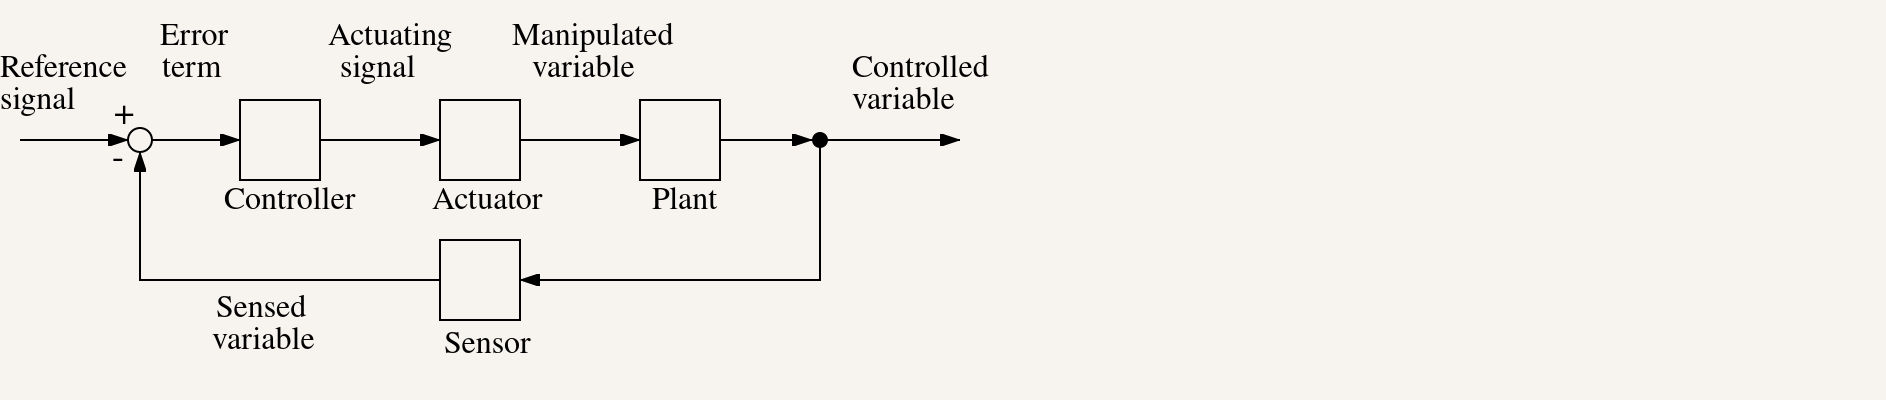
\includegraphics[scale=0.48]{/02/bicycle_feedback_schema}
\caption{Bicycle Feedback Schema}
\label{fig:bicycle_feedback_schema}
\end{figure}

The 'reference signal' or 'set point' is the goal of the system, in this case most likely a
desination and when they want to arrive. The controller takes the set point and the present
conditions, i.e. where the cyclist is currently, the location of obstacles, if the road is heading
uphill or downhill etc.  weather conditions are, how much time they have remaining and convert this
into a control signal. Part of the control signal in this case is observable - the person's
adjustments to the handle-bars, other signals are not observable such as decisions on how hard to
pedal. The actuator in this case is the cyclists leg muscles, which convert those desicions, and use
energy to convert them into pedal pressure. The cyclist then observes the situation again and reacts
to the situation by feeding their sensory data back into the 'controller' and so on in a closed
loop. In the case of the cyclist we depend on continuous inputs in a changing, often unpredictable
environment to adjust behaviour - we require a closed loop system.

\section{History of Control Systems} 

\subsection{Huygens}

\subsection{Watt}

PID controller

\subsection{James Clerk Maxwell}

\subsection{The Wright Brothers}

Prior to the Wright brother's first flight in December 1903, Orville and Wilbur Wright believed that
the most fundamental problems they needed to solve were control problems. In September 1901 Wilbur
Wright's first public presentation on the feasibility of heavier-than-air flight stated that ``When
this one feature [control] has been worked out the age of flying machines will have arrived, for all
other difficulties are of minor importance."\cite{wright1908}

% TODO - this paragraph requires work.

The general view prior to the Wright brothers was that aircraft required the mechanism to
self-stabilize. [this was a problem because incorporating stability into the air-craft was at the
cost of agility. Possibly because the Wright brothers were bicycle-shop owners, and were aware that
bicycles are fundamentally unstable and require human intervention to stay upright, they understood
that this control could be done by the pilot rather than the plane.

\subsection{Elmer Sperry}

Elmer Sperry was the first to construct a PID controller. One notable characteristic of PID
controllers is that despite much work in the design of more sophisticated controllers, PID
controllers are by far the most widely used, demonstrating robustness to solve a broad range of
control problems.

Elmer Sperry is best known for his construction and application of gyroscopes following the
invention of the first practical gyroscope by Hermann Anschütz-Kaempfe in 1904. One of Sperry's
applications was the use of a gyroscope as a component in a control system to self-stabilize
airplanes.

[longer flights]
 
Following on from these experiences, he worked with the U.S. Navy to use gyroscopes for stabilizing
ships, and then also to build control systems as auto-pilots of ships. Because the control process
involved in steering large ships with significant lags and so was relative slow and visible, he was
able to observe that skilled helmsmen used a more nuanced 'algorithm' than just a proportional
response, and that the helmsman with put the helm over in the opposite to the directions in which
the ship was yawing a significantly in advance (a D response), and that helmsman worked the ship
upwards in response to currents and prevailing wind (an I response). Sperry then incorporated these
three responses (P, I and D) into his mechanical control mechanism which connected the gyroscope to
the ships steering.

In 1922 Nicolas Minorsky published a paper which encapsulated the P, I and D into an
equation.\cite{minorsky1922}

\section{Positive Feedback}

\section{Error Correction}

\section{Isolation}

\section{Stability}

\section{The Internet}


